\documentclass[runningheads,a4paper]{llncs}

\usepackage{amssymb}
\usepackage{graphicx}
\usepackage[hidelinks]{hyperref}
\usepackage{enumerate}
\usepackage{multicol}
\usepackage{url}

\setcounter{tocdepth}{3}
\setlength{\columnsep}{2cm}
\urldef{\mailsa}\path|{hbhatt2014}@my.fit.edu|
\newcommand{\keywords}[1]{\par\addvspace\baselineskip
\noindent\keywordname\enspace\ignorespaces#1}
\renewcommand{\baselinestretch}{1.2}

\begin{document}

\mainmatter

\title{Social World Connectivity among the Indian Celebrities}
\titlerunning{Social World Connectivity among the Indian Celebrities}

\author{Harshit Bhatt}
\authorrunning{Social World Connectivity among the Indian Celebrities}

\institute{Florida Institute of Technology, Melbourne 32901.\\
Florida, USA.\\
\mailsa\\
\url{http://www.fit.edu/~hbhatt2014}} 

\maketitle

\begin{abstract}
This work maps social world(twitter) relationship among the verified Indian celebrities and groups based on their mention in tweets. Extracting the data helped in redefining the Inter-Network of the celebrities and gave various facts regarding users(tweeters) affiliation to the celebrities. The whole project helped me to gauge a new perspective of the Indian celebrities in the social media which has not been thought about deeply in the past researches.

\keywords{Twitter API, Social Media, Relationship between Users and Celebrities}
\end{abstract}

\section{Introduction}

\paragraph{}
The main purpose of devising this network was to get an overview of the celebrities fame and their Inter-Network through the Social Media Data. The data here is the tweets, and only those which mention or are related to any of these Celebrities or groups. I have included only those celebrities and groups who are verified from Twitter.

\paragraph{}
Celebrities in the list are from the field of Indian Cinema, Sports and Politics. Due to the popularity of the celebrities among their fan base I was able to collect a large amount of data with the help of Twitter Streaming API.

\paragraph{}
The JSON data given by Twitter API includes a wide range of information about a tweet, which helped in defining the base table for the network, through which I was able to deduce various other meaningful sub-tables which modeled the various networks in my result.

\paragraph{}
Tables which mapped the various graphs were on :

\begin{itemize}

\item List of number of unique users for each celebrity

\item List of common users between each pair of celebrities

\item List of total number of each celebrity mentioned in tweets

\item List of each pair of celebrities who are mentioned in the same tweet and their count

\item List of every user and their mention counts to the celebrity(this list is for each celebrity)

\item List containing hashtags related to celebrities

\item List having common hashtags reference between the celebrities

\end{itemize}

\paragraph{}
There were three networks that were constructed with these tables and their result has been shown in the Result section of this report. The networks had lot of edges between them which I reduced with the filters in Gephi to get a common overview of the network so only the most prominent nodes were left in the network. The nodes size was taken in accordance to their Betweenness Centrality as it gives a more real dominance of the nodes in the network, the edge strength is the number of relations between the celebrities, more thick edge means more those celebrities are related to each other. Each node is also provided with its Meta Data which include celebrities twitter handle. The network structure is developed through OpenOrd layout of Gephi with node color and community division done in accordance to the modularity class.

\paragraph{}
With help of Gephi I was able to calculate Degree distribution, Betweenness and Closeness centrality, Eccentricity and Modularity of the network whose result I have shown in the Result section for further detailed study of the networks.

\section{Building the Twitter Network}

\begin{itemize}

\item The first step was to set up Twitter Streaming API which was processed by getting my special token and secret key from twitter for this application.

\item The python library Tweepy was used as a bridge to collect tweets from the Twitter Inc.

\item The whole program is set up in the Python language, which helped to collect tweets and its other relevant information, which was further saved into MySQL database tables so as to map the networks.

\item The main/initial table for the network is named celebrity\_tweets which includes the data that is collected directly from the tweets.

\item Its fields are -$>$

\subitem	user\_twitter\_id  -$>$  it has the twitter id of the person who has send that tweet.
\subitem	user\_name  -$>$  user twitter handle.
\subitem	tweet  -$>$  the actual tweet which has been sent by the user.
\subitem	users\_mention\_id  -$>$  twitter id of the celebrities that are mentioned in the tweet.
\subitem	hashtags -$>$ hashtags that are in the tweet and are related to those celebrities. 

\item	To get all (most of) the celebrities in India I first choose four most famous Indian celebrities(based on general prospective) which by their twitter handle are @SrBachchan, @iamsrk, @msdhoni, @pmoindia.

\item	With the help of Twitter Streaming API I was able to collect all the Verified friends and friends of friends of these four celebrities.

\item	Friends details of these four celebrities and their friends were saved in their respective named tables(eg. iamsrk\_friends) with table having fields as :

\subitem	user\_id  -$>$  celebrity twitter id
\subitem	user\_name -$>$ celebrity twitter handle

\item	Now a list was made to remove the duplicates from these tables and get a unique list of celebrities.

\item This list was saved to a table named celebrities which holds detail for every celebrity used in our tweet collection. It has fields as :

\subitem	celebrity\_twitter\_id  -$>$  celebrity twitter id
\subitem	celebrity\_twitter\_name -$>$ celebrity twitter handle

\item	There were total of 467 unique celebrities and verified groups which I finally got as the input for data collection.

\item	The program is now executed with the input of these unique celebrities.

\item	The data collected is saved in the celebrity\_tweets table as discussed above.

\item Only those tweets were collected which have either hashtags with celebrities mentioned or only celebrities mentioned or tweets from these celebrities having hashtags.

\item	The data was collected within a range of 23 days and total tweets collected were 361,296.

\item	After the data collection some relevant tables were deduced from the main table, which were respectively related to the specific networks which we have mapped to show the final results.
\vspace{0.1in}
\item There were Six tables deduced namely : 
\vspace{0.1in}
\subitem	a. celebrity\_mentions\_count -$>$ this table stores the total mentions which a celebrity received during the time period. It has fields as : 

\begin{enumerate}[i.  ]
\addtolength{\itemindent}{1cm}
\item celebrity\_twitter\_id -$>$ celebrity twitter id
\item nodes -$>$ celebrity twitter handle
\item weight -$>$ total user mentions
\end{enumerate}
\vspace{0.1in}
\subitem b. celebrity\_common\_mention\_tweets -$>$ this table gives the number of tweets in which the celebrities are commonly mentioned. It has fields as :

\begin{enumerate}[i.  ]
\addtolength{\itemindent}{1cm}
\item source -$>$ one of the celebrities twitter handle in the pair
\item celebrity1\_id -$>$ first celebrity twitter id
\item target -$>$ the other celebrity twitter handle in the pair
\item celebrity2\_id -$>$ second celebrity twitter id
\item weight -$>$ number of tweets having celebrities common mentioned
\end{enumerate}
\vspace{0.1in}
\subitem  c. celebrity\_specific\_distinct\_hashtags\_count -$>$ this table gives the total number of different hashtags that are connected to the celebrity. It has fields as :

\begin{enumerate}[i.  ]
\addtolength{\itemindent}{1cm}
\item celebrity\_twitter\_id -$>$ celebrity twitter id
\item nodes -$>$ celebrity twitter handle
\item weight -$>$ total distinct hashtags connected with the celebrity
\end{enumerate}
\vspace{0.1in}
\subitem d. celebrity\_hashtags\_common -$>$ this table gives the number of hashtags that are common between each pair of celebrities. It has fields as :

\begin{enumerate}[i.  ]
\addtolength{\itemindent}{1cm}
\item source -$>$ one of the celebrities twitter handle in the pair
\item celebrity1\_id -$>$ first celebrity twitter id
\item target -$>$ the other celebrity twitter handle in the pair
\item celebrity2\_id -$>$ second celebrity twitter id
\item weight -$>$ number of hashtags that are common between them
\end{enumerate}
\vspace{0.1in}
\subitem e. celebrity\_number\_unique\_users -$>$ this table gives the total unique users that a celebrity got mentioned by. It has fields as :

\begin{enumerate}[i.  ]
\addtolength{\itemindent}{1cm}
\item celebrity\_twitter\_id -$>$ celebrity twitter id
\item nodes -$>$ celebrity twitter handle
\item weight -$>$ number of unique users for the celebrity
\end{enumerate}
\vspace{0.1in}
\subitem f. celebrity\_users\_common -$>$ this table gives the number of users that are common between each pair of celebrities. It has fields as :

\begin{enumerate}[i.  ]
\addtolength{\itemindent}{1cm}
\item source -$>$ one of the celebrities twitter handle in the pair
\item celebrity1\_id -$>$ first celebrity twitter id
\item target -$>$ the other celebrity twitter handle in the pair
\item celebrity2\_id -$>$ second celebrity twitter id
\item weight -$>$ number of users that are common between them
\end{enumerate}

\item	I have also saved the users details, it contains information on twitter users who have mentioned the celebrities in another database with tables name as of the celebrity name containing the fields as : 
  
\subitem user\_id -$>$ user twitter id who has mentioned that celebrity
\subitem user\_name -$>$ users twitter handle
\subitem count -$>$ number of times that celebrity has been mentioned by the user

\item	Three networks were constructed with the help of the above six tables. With help of igraph python library and Gephi Software I was able to map these networks. The networks are as following : 
\vspace{0.1in}
\subitem	a. The first network uses celebrity\_users\_common and celebrity\_number\_unique\_users tables to generate a relationship which proposes the common users between each pair of celebrities, in this network :
\vspace{0.1in}
\begin{enumerate}[i.  ]
\addtolength{\itemindent}{1cm}
\item Nodes -$>$ Celebrities
\item Node Size -$>$ Betweenness Centrality of the node
\item Edges -$>$ Common Users between Celebrities
\item Edge Strength -$>$ Common Users count
\end{enumerate}
\vspace{0.1in}
\textbf{For example =$>$}
\begin{flushleft}
\centerline{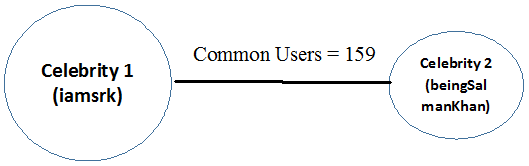
\includegraphics[width=0.7\textwidth,height=0.5\textheight,keepaspectratio]{common_users_eg_1.png}}
\centerline{Unique Users = 6353 \hspace{2cm} Unique Users = 852}
\vspace{0.2in}
\centerline{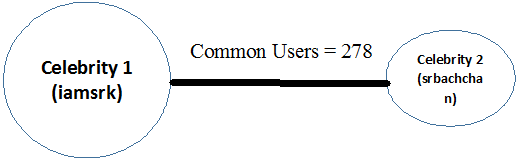
\includegraphics[width=0.7\textwidth,height=0.5\textheight,keepaspectratio]{common_users_eg_2.png}}
\centerline{Unique Users = 6353 \hspace{2cm} Unique Users = 797}
\end{flushleft}
\subitem b. The second network uses celebrity\_mentions\_count and celebrity\_common\_mention\_tweets tables to generate a relationship which proposes how commonly two celebrities are mentioned in the same tweets, in this network :
\vspace{0.1in}
\begin{enumerate}[i.  ]
\addtolength{\itemindent}{1cm}
\item Nodes -$>$ Celebrities
\item Node Size -$>$ Betweenness Centrality of the node
\item Edges -$>$ Celebrities common in tweets
\item Edge Strength -$>$ count of Celebrities common mentions
\end{enumerate}
\vspace{0.1in}
\textbf{For example =$>$}
\begin{flushleft}
\centerline{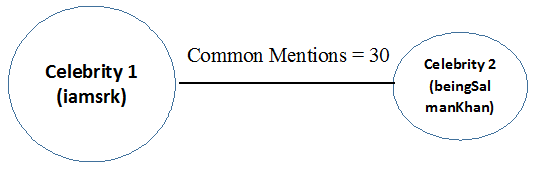
\includegraphics[width=0.7\textwidth,height=0.5\textheight,keepaspectratio]{common_mention_eg_1.png}}
\centerline{Total Mentions = 23443 \hspace{2cm} Total Mentions = 1693}
\vspace{0.2in}
\centerline{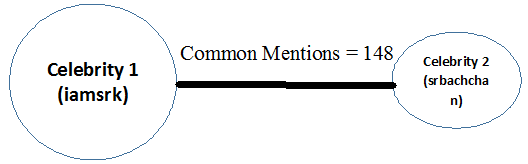
\includegraphics[width=0.7\textwidth,height=0.5\textheight,keepaspectratio]{common_mention_eg_2.png}}
\centerline{Total Mentions = 23443 \hspace{2cm} Total Mentions = 1087}
\end{flushleft}
\subitem c. The third network uses celebrity\_specific\_distinct\_hashtags\_count and celebrity\_hashtags\_common tables to generate a relationship which proposes how many hashtags are common between the celebrities, in this network :
\vspace{0.1in}
\begin{enumerate}[i.  ]
\addtolength{\itemindent}{1cm}
\item Nodes -$>$ Celebrities
\item Node Size -$>$ Betweenness Centrality of the node
\item Edges -$>$ Celebrities common hashtags
\item Edge Strength -$>$ count of Celebrities common hashtags
\end{enumerate}
\vspace{0.1in}
\textbf{For example =$>$}
\begin{flushleft}
\centerline{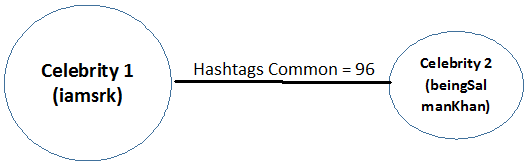
\includegraphics[width=0.7\textwidth,height=0.5\textheight,keepaspectratio]{common_hashtags_eg_1.png}}
\centerline{Total Mentions = 1165 \hspace{2cm} Total Mentions = 276}
\vspace{0.2in}
\centerline{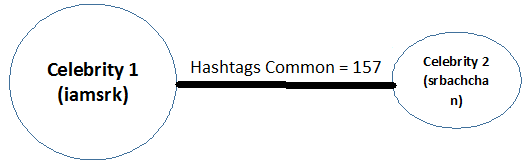
\includegraphics[width=0.7\textwidth,height=0.5\textheight,keepaspectratio]{common_hashtags_eg_2.png}}
\centerline{Total Mentions = 1165 \hspace{2cm} Total Mentions = 376}
\end{flushleft}

\item For better viewing these networks were exported to GraphML format and were then viewed in Gephi, to divide the network into clusters OpenOrd layout was chosen, to further divide them into communities Modularity algorithm of Gephi was used, the nodes were colored with their respective modularity class color which made it easy to distinguish the nodes.

\item The networks were highly cluttered due to large number of edges(2216,21978,22188), hence to make them more viewable I applied Gephi filters of degree range and edge weight range which choose edges above certain weight(20,20,15) and nodes having degree 1 or more, this made some nodes to disappear but still the network gives a generalization of the relationships.  

\end{itemize}

\section{Related Work}

\paragraph{}
Many such networks regarding the relationships among celebrities have been developed in the past by researchers. As the celebrities hold special status in general public mind, hence their demeanor, their activities, their words affect people deeply, which made researchers to work on this field as it encloses within it vast opportunities. Hence, there has been many research$'$s regarding this relationship but I would be here concentrating upon three main research$'$s which made me to opt for this topic.
\paragraph{}
Most of the research in this field is based on the public database of IMDb which include actors and their movies and when they have worked with each other, which helps to construct a relationship between the celebrities. The three networks were : 
\subsection{Fafadia Tech Blog}
There has been no such research on Indian celebrities social media relationship in the past which made me to delve into this field. My main inspiration comes from a surprising source - a blog which I read while surfing on the internet of Fafadia Tech \cite{fafadia} where they have shown a relationship between the Indian actors on the context of those celebrities working together in the year 2013, the data for which they got from the IMDb public database but I tried to extend that work by taking Social Media in the context and using real world common public tweets for drawing a relation between these celebrities which could show a more genuine relationship between the Indian celebrities.
\subsection{Movies and Actors in Hollywood}
Another work related to the affiliation between the Movies and Actors in Hollywood was done by Herr, Ke, Hardy, Borner in 2007 \cite{1} where they conducted the same experiment as above for the actors and their affiliation with the movies they have worked on, using the information from IMDb public database. They focused their research on the movies produced between 1890 to 2007 with co-actors network following it. They finally superimposed both these networks on top of each other to get a final network which includes movie name, when it was made and actors who worked in it. The co-actor network includes the relationship among all the actors who have worked with each other in these movies, they nodes are actors with edges showing the strength of their relationship which tells about how many movies they have worked in with each other. The final network had movies distinguished based on their genre with actors receiving the color depending on the genre of movies they have most worked in.
\subsection{Analysis and Measurement of Social Media}
One other work related to the analysis and measurement of social network \cite{2} also helped me to finalize the basic theme and initial setup of my network where Mislove, Marcon, Gummadi, Druschel, Bhattacharjee 2007 have shown how does the social network has been and could be used as a genuine medium for measuring various real world entities in the near future as more and more people are now concentrating on this medium for communicating and expressing their thoughts and ideas. Their work was done between the year 2005-2007 where they concentrated their research on four of the top social networking sites at that time(Flickr,YouTube,Orkut,Live Journal). Their study was vast with around 11.3 million users having 328 million links. Their research tried to find the similar interest among the users and the resources that have been mostly shared by them. By getting to know about this information they were able to deduce the basic structure of Social Media and how it works. They also predicted social media functionality in the future, they proposed that as social media continues to grow it would account for the majority of Web traffic and as more people would be joining this network it becomes important to know about their behavior, which in turn could help to provide them a more feasible and related social media structure and this study could also help in improving security of the networks as well as the internet.
\paragraph{}
I would like to extend this study to include the sentimental analysis of tweets, which would help to get the idea on how does the general public consider the celebrities. This metric could help in deciding the celebrity status and give us the fact that whether their image is positive or negative in general public mind. Similarly I could also have made a bipartite network between celebrities - twitter users and celebrities - hashtags to get more specific information on this relationship but due to time constraint I have skipped these options for future.

\section{Experimental Results}

\centerline{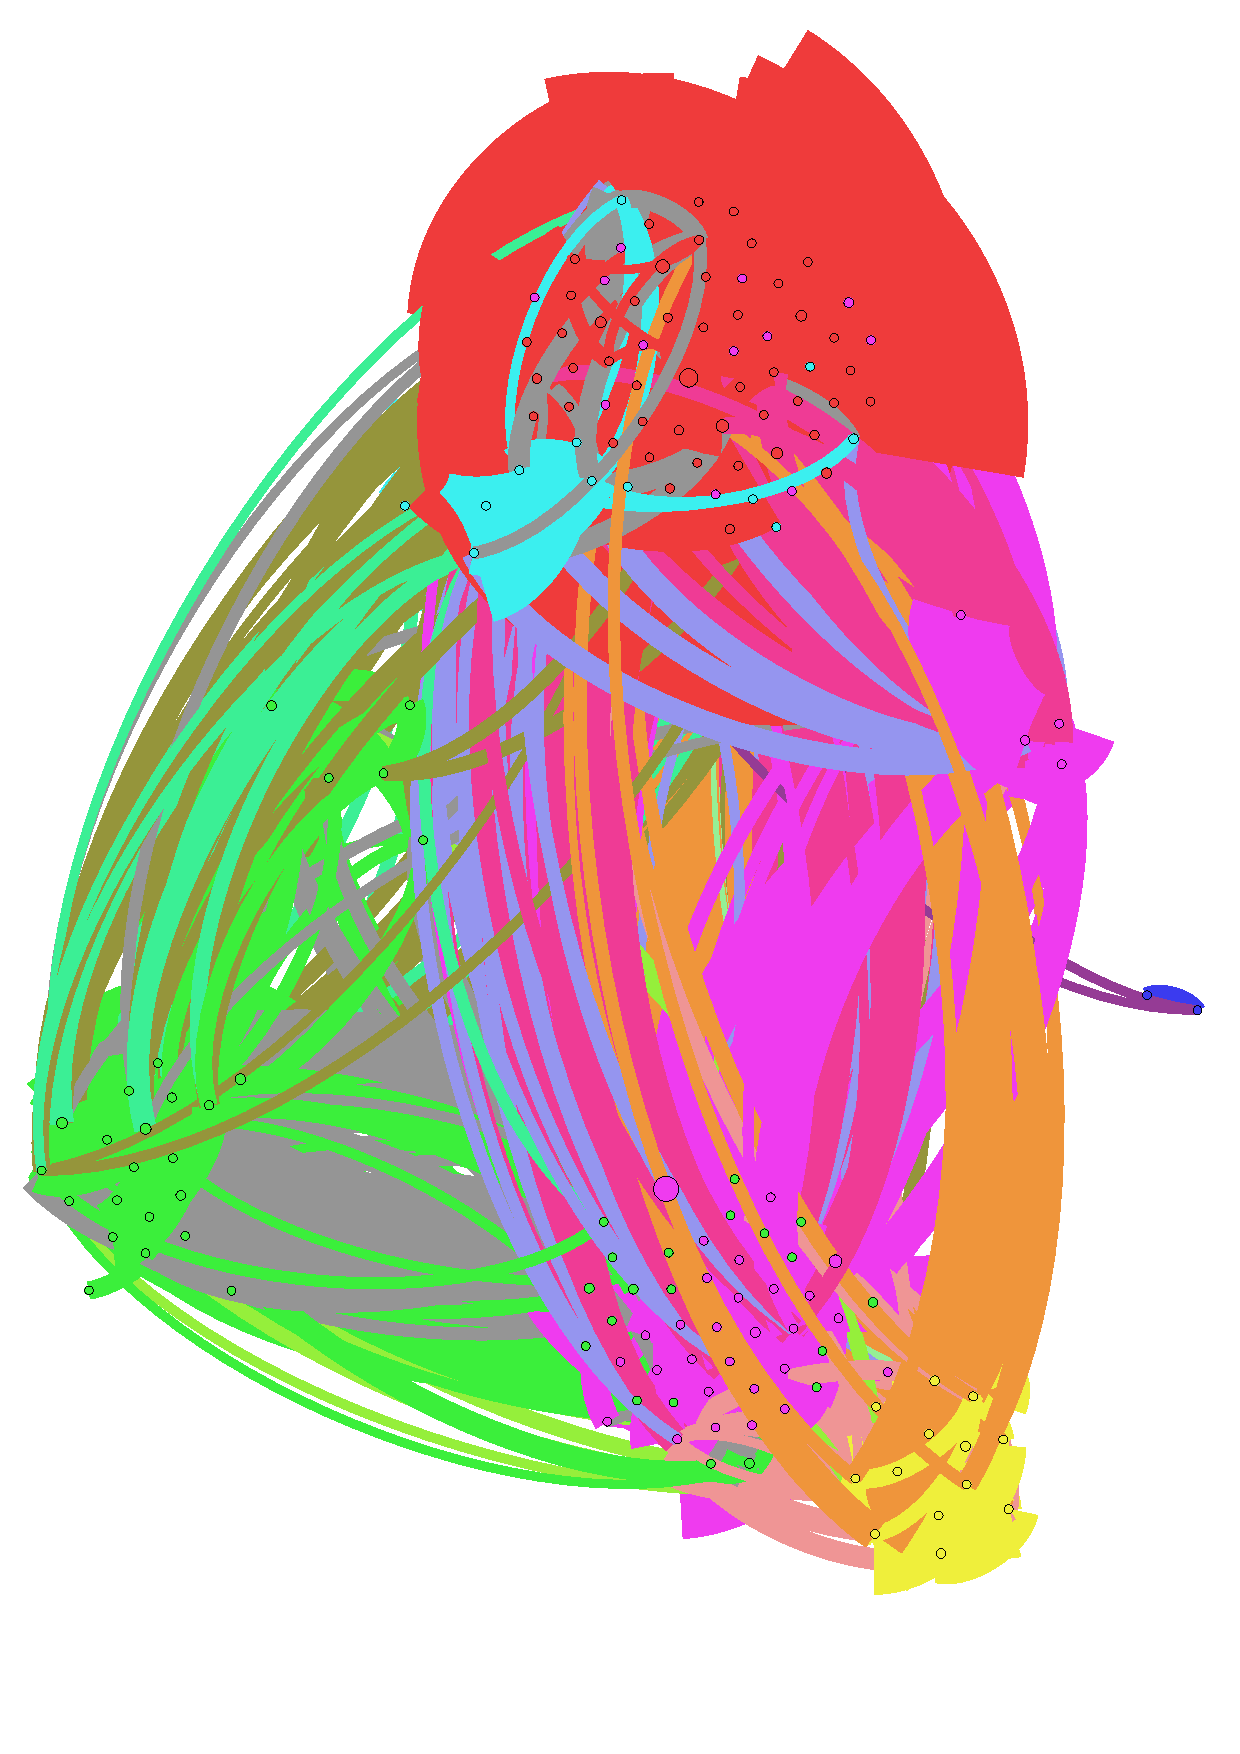
\includegraphics[width=\textwidth,height=\textheight,keepaspectratio]{users_common_network.png}}
\vspace{0.1in}
\centerline{Common Users between Celebrities Community Network}
\vspace{0.2in}
\noindent{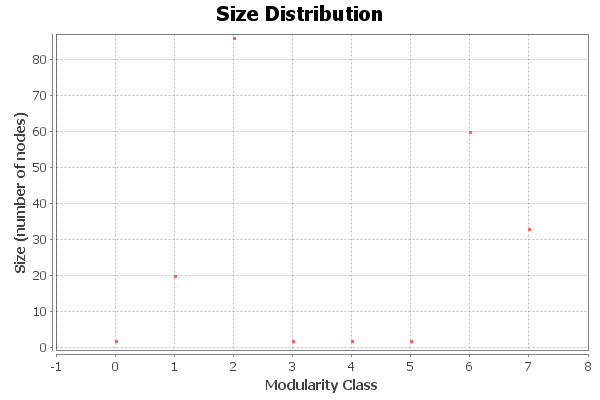
\includegraphics[width=0.45\textwidth,height=0.5\textheight,keepaspectratio]{users_common_modularity_graph.png}}\hspace{1.2cm}
\noindent{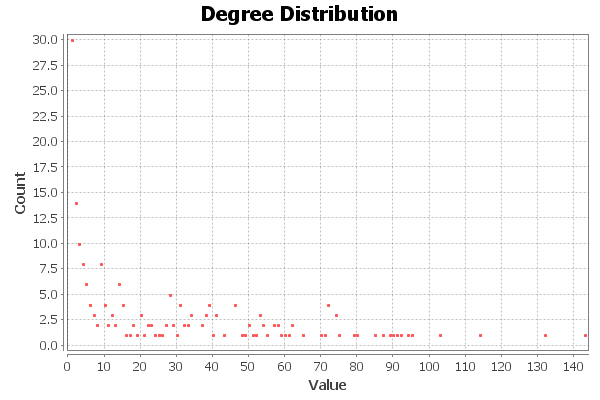
\includegraphics[width=0.45\textwidth,height=0.5\textheight,keepaspectratio]{users_common_degree_graph.png}}
\vspace{-0.5cm}
\begin{multicols}{2}{\noindent{Graph for the Communities Distribution of Common Users Network}}\vfill\columnbreak{\noindent{Graph for the Degree Distribution of Common Users Network}}\end{multicols}
\vspace{-0.5cm}
\begin{multicols}{2}{\noindent{\fontsize{10}{12}{\textbf{Results =$>$ Modularity: 0.351, Number of Communities: 8}}}}\vfill\columnbreak{\noindent{\fontsize{10}{12}{\textbf{Results =$>$ Average Degree: 26.947}}}}\end{multicols}
\vspace{-0.4cm}
\noindent{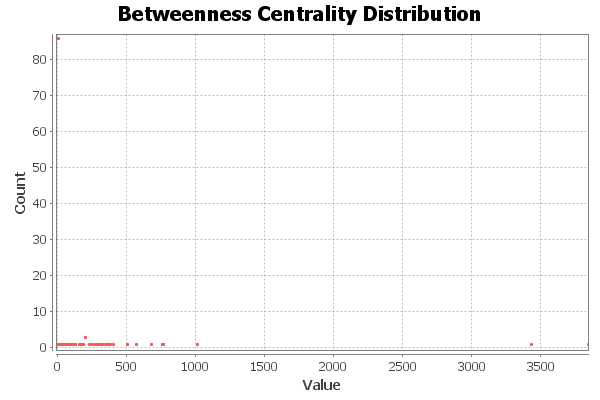
\includegraphics[width=0.45\textwidth,height=0.5\textheight,keepaspectratio]{users_common_betweenness_graph.png}}\hspace{1.2cm}
\noindent{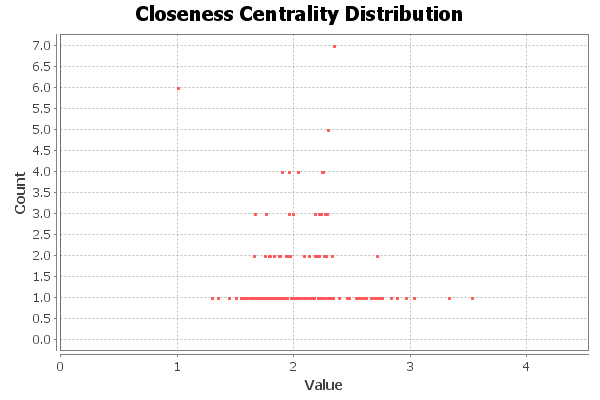
\includegraphics[width=0.45\textwidth,height=0.5\textheight,keepaspectratio]{users_common_closeness_graph.png}}
\vspace{-0.5cm}
\begin{multicols}{2}{\noindent{Graph for Betweenness Centrality Distribution of Common Users Network}}\vfill\columnbreak{\noindent{Graph for Closeness Centrality Distribution of Common Users Network}}\end{multicols}
\vspace{-0.2cm}
\centerline{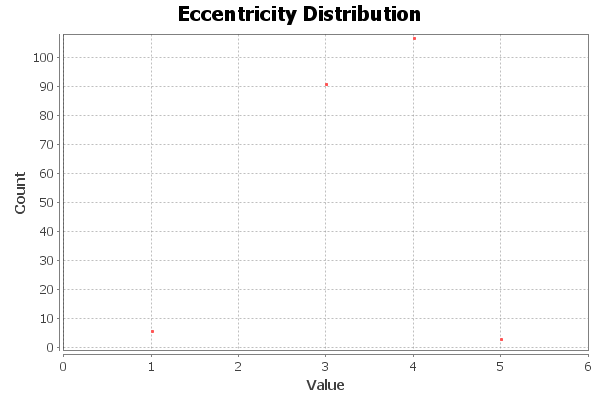
\includegraphics[width=0.5\textwidth,height=0.5\textheight,keepaspectratio]{users_common_eccentricity_graph.png}}
\centerline{Graph for Eccentricity Distribution of Common Users Network}
\vspace{0.2in}
\centerline{\fontsize{10}{12}{\textbf{Results =$>$ Diameter: 5, Radius: 1, Average Path length: 2.0907, Number of shortest paths: 40206}}}
\vspace{0.2in}
\centerline{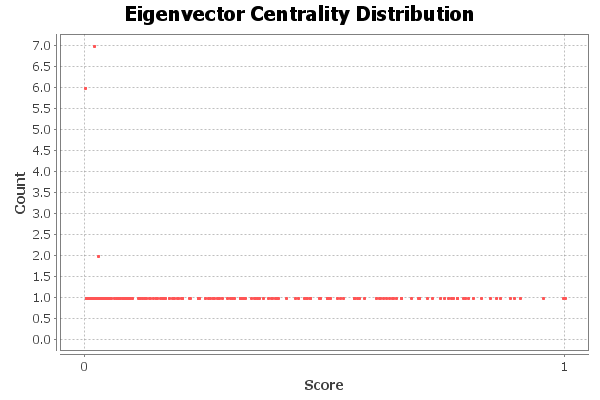
\includegraphics[width=0.5\textwidth,height=0.5\textheight,keepaspectratio]{users_common_eigenvector_graph.png}}
\centerline{Graph for EigenVector Centrality Distribution of Common Users Network}
\vspace{0.2in}
\centerline{\fontsize{10}{12}{\textbf{Parameters =$>$ Number of iterations: 100, Sum change: 0.006464}}}

\begin{figure}
\centering
\includegraphics[width=\textwidth,height=\textheight,keepaspectratio]{common_mention_network.png}
\caption{Celebrities mention in same tweet Community Network}
\end{figure}

\begin{figure}
\noindent{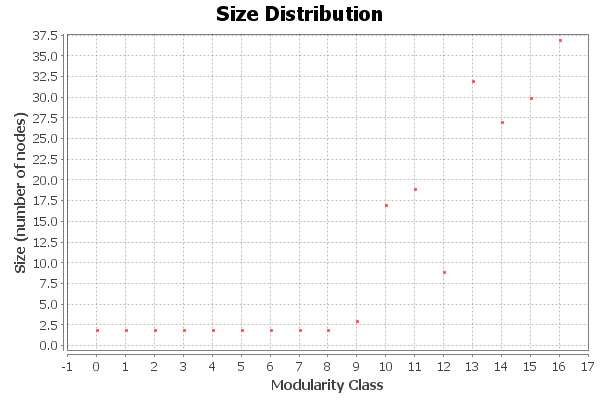
\includegraphics[width=0.45\textwidth,height=\textheight,keepaspectratio]{common_mention_modularity_graph.png}}\hspace{1.2cm}{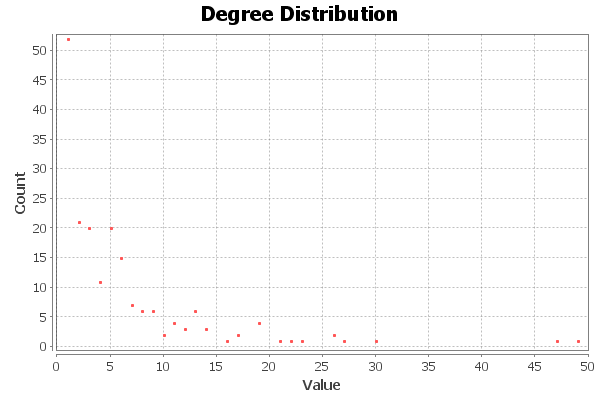
\includegraphics[width=0.45\textwidth,height=\textheight,keepaspectratio]{common_mention_degree_graph.png}}
\begin{multicols}{2}{\caption{Graph for the Communities Distribution of Common Mention Network}}\vfill\columnbreak{\caption{Graph for the Degree Distribution of Common Mention Network}}\end{multicols}
\begin{multicols}{2}{\noindent{\fontsize{10}{12}{\textbf{Results =$>$ Modularity: 0.580, Number of Communities: 17}}}}\vfill\columnbreak{\noindent{\fontsize{10}{12}{\textbf{Results =$>$ Average Degree: 6.021}}}}\end{multicols}
\end{figure}

\begin{figure}
\noindent{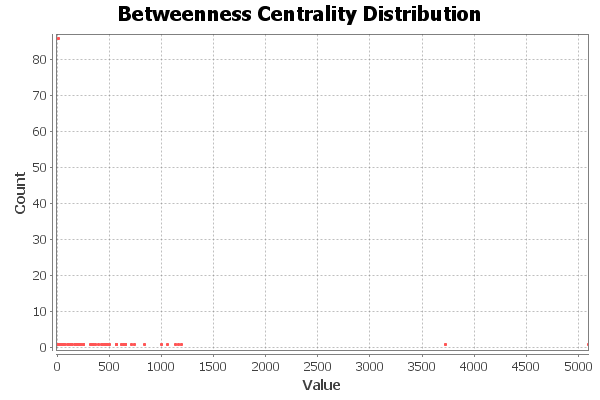
\includegraphics[width=0.45\textwidth,height=\textheight,keepaspectratio]{common_mention_betweenness_graph.png}}\hspace{1.2cm}{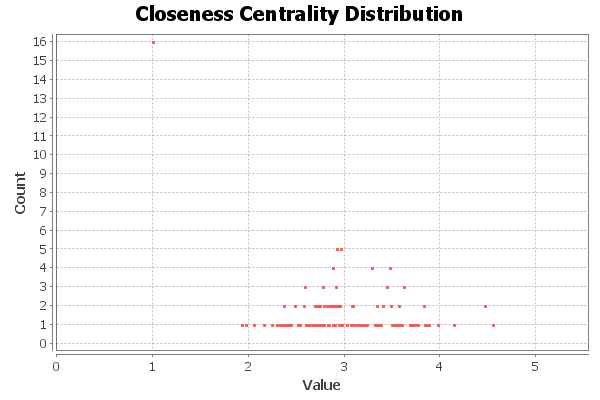
\includegraphics[width=0.45\textwidth,height=\textheight,keepaspectratio]{common_mention_closeness_graph.png}}
\begin{multicols}{2}{\caption{Graph for Betweenness Centrality Distribution of Common Mention Network}}\vfill\columnbreak{\caption{Graph for Closeness Centrality Distribution of Common Mention Network}}\end{multicols}
\end{figure}

\begin{figure}
\centerline{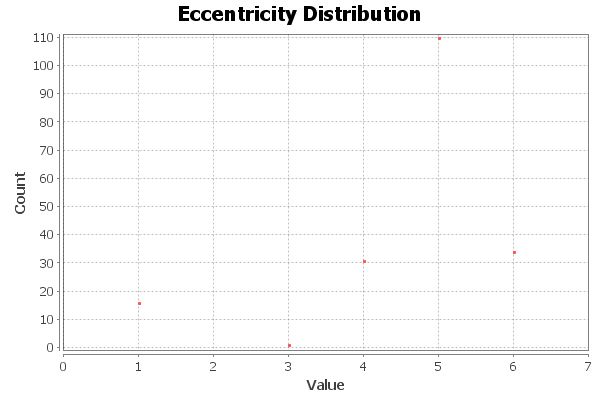
\includegraphics[width=0.50\textwidth,height=\textheight,keepaspectratio]{common_mention_eccentricity_graph.png}}
\caption{Graph for Eccentricity Distribution of Common Mention Network}
\vspace{0.1in}
\centerline{\fontsize{10}{12}{\textbf{Results =$>$ Diameter: 6, Radius: 1, Average Path length: 3.0195, Number of shortest paths: 30816}}}
\end{figure}

\begin{figure}
\centerline{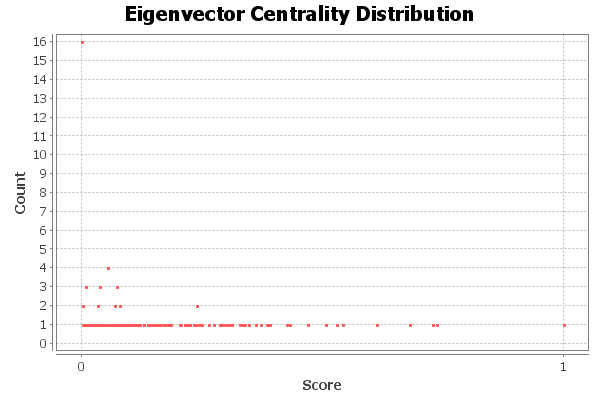
\includegraphics[width=0.5\textwidth,height=\textheight,keepaspectratio]{common_mention_eigenvector_graph.png}}
\caption{Graph for EigenVector Centrality Distribution of Common Mention Network}
\vspace{0.1in}
\centerline{\fontsize{10}{12}{\textbf{Parameters =$>$ Number of iterations: 100, Sum change: 0.007861}}}
\end{figure}

\begin{figure}
\centering
\includegraphics[width=\textwidth,height=\textheight,keepaspectratio]{hashtags_common_network.png}
\caption{Common Hashtags between Celebrities Community Network}
\end{figure}

\begin{figure}
\noindent{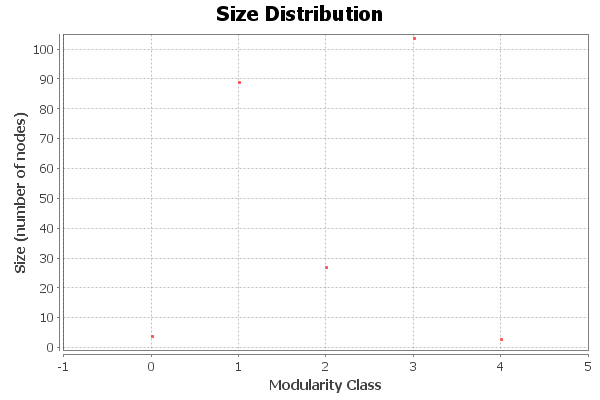
\includegraphics[width=0.45\textwidth,height=\textheight,keepaspectratio]{hashtags_common_modularity_graph.png}}\hspace{1.2cm}{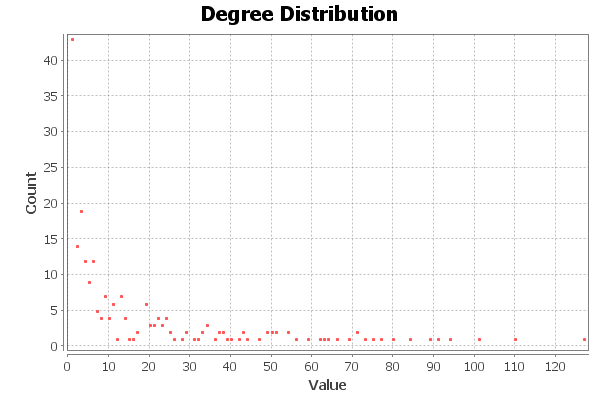
\includegraphics[width=0.45\textwidth,height=\textheight,keepaspectratio]{hashtags_common_degree_graph.png}}
\begin{multicols}{2}{\caption{Graph for the Communities Distribution of Common Hashtags Network}}\vfill\columnbreak{\caption{Graph for the Degree Distribution of Common Hashtags Network}}\end{multicols}
\begin{multicols}{2}{\noindent{\fontsize{10}{12}{\textbf{Results =$>$ Modularity: 0.315, Number of Communities: 5}}}}\vfill\columnbreak{\noindent{\fontsize{10}{12}{\textbf{Results =$>$ Average Degree: 18.106}}}}\end{multicols}
\end{figure}

\begin{figure}
\noindent{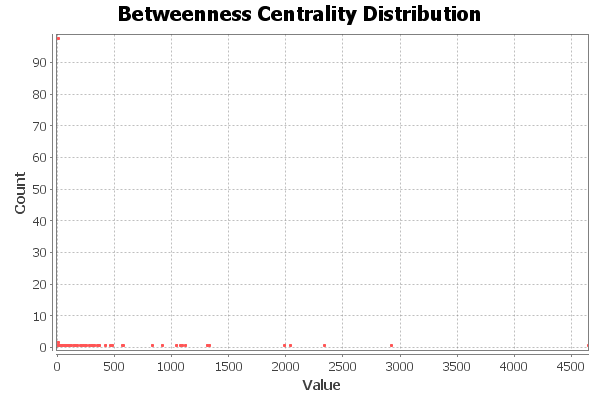
\includegraphics[width=0.45\textwidth,height=\textheight,keepaspectratio]{hashtags_common_betweenness_graph.png}}\hspace{1.2cm}{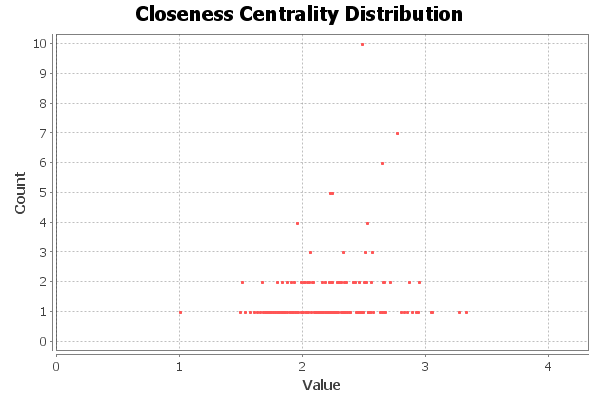
\includegraphics[width=0.45\textwidth,height=\textheight,keepaspectratio]{hashtags_common_closeness_graph.png}}
\begin{multicols}{2}{\caption{Graph for Betweenness Centrality Distribution of Common Hashtags Network}}\vfill\columnbreak{\caption{Graph for Closeness Centrality Distribution of Common Hashtags Network}}\end{multicols}
\end{figure}

\begin{figure}
\centerline{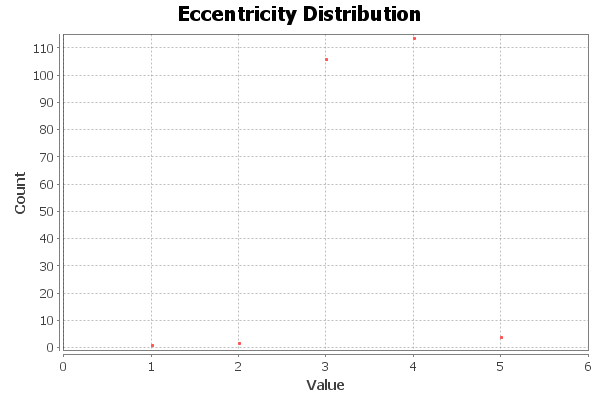
\includegraphics[width=0.50\textwidth,height=\textheight,keepaspectratio]{hashtags_common_eccentricity_graph.png}}
\caption{Graph for Eccentricity Distribution of Hashtags Common Network}
\vspace{0.1in}
\centerline{\fontsize{10}{12}{\textbf{Results =$>$ Diameter: 5, Radius: 1, Average Path length: 2.2723, Number of shortest paths: 49958}}}
\end{figure}

\begin{figure}
\centerline{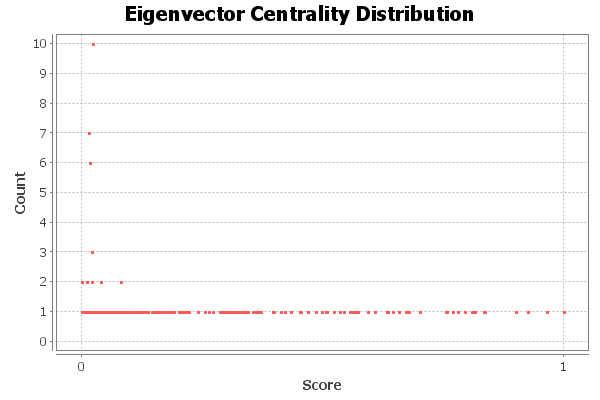
\includegraphics[width=0.5\textwidth,height=\textheight,keepaspectratio]{hashtags_common_eigenvector_graph.png}}
\caption{Graph for EigenVector Centrality Distribution of Common Hashtags Network}
\vspace{0.1in}
\centerline{\fontsize{10}{12}{\textbf{Parameters =$>$ Number of iterations: 100, Sum change: 0.004076}}}
\end{figure}

\section{Conclusion}

\paragraph{}
After analyzing the three networks we get to know about the strength(count) of the users relationship with the celebrities and who are the celebrities that tweeters consider most related to each other and with themselves.

\paragraph{}
We also get to know from the collected data about the users who tweet most on celebrities and whether or not they are loyal to one celebrity or many.

\paragraph{}
My study shows that as in accordance to the general perspective the social media also shows the same relationship among the celebrities, making the celebrities from the same community(politics, cinema and sport) to be related more to each other than with other community and the users being more common between those community celebrities. Surely there are some exceptions but they are overshadowed by the strong relation between the celebrities in single community.

\paragraph{}
For the common users network there were 8 different communities with modularity of 0.351, in this network two clusters were prominent which constitute mostly actors with their related entertainment groups(brown) and politicians with news channels and Government organizations in other(green), the third celebrity group of sport stars were mixed in both these groups and were less in number as compare to other two groups. Surely some communities such as(violet) has some mix of celebrities such as sport stars and actors, this community has Indian Super League(@IndSuperLeague)(soccer event) as the central node, and the celebrities are team owners with other nodes as participating teams. Other smaller isolated clusters(green,blue) are also connected to each other with their current involvement specific to each other. Within this network two nodes stood out(@narendramodi and @iamsrk) due to their highest Betweenness centrality in the two respective big clusters which gives us the conclusion that these two celebrities are most mentioned by the users and most of the other celebrities within those clusters have users common with these two. There were some movie stars present in the politicians cluster with strong relationship, which proves the goal for designing this network as we could deduce that some of the tweeting population takes interest in both politics and movies simultaneously.

\paragraph{}
For the common mention tweets, the network is more spatial and diverse with 17 communities and modularity of 0.580, even here there are two major clusters with same two celebrities(@narendramodi and @iamsrk) having main clout due to their high Betweenness centrality, but here due to large number of communities there are some other relevant groups like(violet) of @aamaadmiparty and its members which suggests that these members are more mentioned with each other in a tweet than with others. A single community member(@suhelseth)(violet) strikes out prominently due to his common mention with many other celebrities which is a surprise element in this network. Other isolated communities are also present which is due to the celebrities in them being commonly mention with each other prominently, due to which we could see the large number of communities. This network could be considered as explaining the real nature of associativity between the celebrities. This network largely differs from the one above, and hence we could conclude that although a twitter user tweets mentioning celebrities from different genres but only those celebrities are mentioned with each other in a tweet by users who either work with each other or share some common events. Another striking discovery in this network is that @narendramodi Indian Prime minister is more commonly mentioned with some Movie stars than his colleagues. Another feature of the network is that the connection among the movie stars is far more stronger than the politicians.

\paragraph{}
The third network on the common hashtags between celebrities has 5 communities with modularity 0.315, is more concentrated and could be easily seen to be divided in three major clusters. This network is vastly different from the other two networks as here the three main celebrities due to their Betweenness centrality are(@ibnlive, @deepikapadukone and @sonamkapoor) which is different from the previous one's and are quite surprising which holds out that these celebrities are mostly mentioned with the hashtags, with most of the other celebrities connected to them. Here a third community(red) is also prominent cluster which contains more of sport celebrities connected with each other due to Indian Super League(@IndSuperLeague) event with inclusion of some actors as well which shows that these actors have more hashtags common with the sport stars than their own group of people, which holds the theory true that celebrities are connected to each other not merely on their field of work but due to the events they are involved in.

\paragraph{}
Some celebrities or organizations have a very large number of mentions than others which may be due to those celebrities(politicians, sport and movie stars) being trending in India for some cause (movie release, an event being taking place or due to their certain initiatives) examples of which could be given with @iamsrk, @deepikapadukone movie stars mentioned a lot due to their movie released within this time period or @IndSupLeague an organization which is conducting a football event within India during this time or @narendramodi India Prime Minister for starting a cleanliness drive campaign within the country.

\paragraph{}
The common mention between some celebrities also has some great numbers like for @iamsrk, @deepikapadukone, @juniorbachchan, @farahkhan are mentioned a great number of times with each other due to a movie release which had all of them working together. The same was for the teams like @FCGoa, @atlidkolkata, @PuneFC and others due to their involvement in a league.

\paragraph{}
Taking all three networks in consideration finally I could say that the celebrity which stood out in the whole network is(@narendramodi) India's Prime Minister as he has been the most prominent player in all three networks which comes out as a great signal for India as this means most of the celebrities and tweeting community relate to the supreme power of the country which should help in smooth and fair Governance as it has the inclusion of most of the public, it also provide great prospects for India as people are more united and relate to the works of Government.

\paragraph{}
Finally I could say that if popularity could be gauged by the mention of celebrities it would hold true to what general perspective is. Still as a caveat before considering this study as the real truth among celebrities relationship is that the study is solely based on the social media mention of celebrities and has been done for a short period of time if the research could be extended to a different level it could be validated to some extent with the real world.

\begin{thebibliography}{3}

\bibitem{1} \href{http://nwb.cns.iu.edu/papers/2007-herr-movieact.pdf}Movies and Actors : Mapping the Internet Movie Database - Bruce W. Herr, Katy Borner, Weimao Ke, Elisha Hardy. 2007
\vspace{0.1in}
\bibitem{2} \href{http://www.mpi-sws.org/~mmarcon/SocialNetworks-IMC.pdf}Measurement and Analysis of Online Social Networks - Alan Mislove, Peter Druschel, Massimiliano Marcon, Krishna P. Gummadi, Bobby Bhattacharjee. 2007
\vspace{0.1in}
\bibitem{fafadia} \href{https://github.com/sidharthshah/bollywood-social-network-analysis}Fafadia Tech Blog. 2014

\end{thebibliography}

\end{document}
